\documentclass[compress]{beamer}
\usepackage{ifthen,verbatim}

\newcommand{\isnote}{}
\xdefinecolor{lightyellow}{rgb}{1.,1.,0.25}
\xdefinecolor{darkblue}{rgb}{0.1,0.1,0.7}

%% Uncomment this to get annotations
%% \def\notes{\addtocounter{page}{-1}
%%            \renewcommand{\isnote}{*}
%% 	   \beamertemplateshadingbackground{lightyellow}{white}
%%            \begin{frame}
%%            \frametitle{Notes for the previous page (page \insertpagenumber)}
%%            \itemize}
%% \def\endnotes{\enditemize
%% 	      \end{frame}
%%               \beamertemplateshadingbackground{white}{white}
%%               \renewcommand{\isnote}{}}

%% Uncomment this to not get annotations
\def\notes{\comment}
\def\endnotes{\endcomment}

\setbeamertemplate{navigation symbols}{}
\setbeamertemplate{headline}{\mbox{ } \hfill
\begin{minipage}{5.5 cm}
\vspace{-0.75 cm} \small
\end{minipage} \hfill
\begin{minipage}{4.5 cm}
\vspace{-0.75 cm} \small
\begin{flushright}
\ifthenelse{\equal{\insertpagenumber}{1}}{}{Jim Pivarski \hspace{0.2 cm} \insertpagenumber\isnote/\pageref{numpages}}
\end{flushright}
\end{minipage}\mbox{\hspace{0.2 cm}}\includegraphics[height=1 cm]{../cmslogo} \hspace{0.1 cm} \includegraphics[height=1 cm]{../tamulogo} \hspace{0.01 cm} \vspace{-1.05 cm}}

\begin{document}
\begin{frame}
\vfill
\begin{center}
\textcolor{darkblue}{\Large Update in Understanding the ``Sawtooth'' Effect}

\vfill
\begin{columns}
\column{0.3\linewidth}
\begin{center}
\large
\textcolor{darkblue}{Jim Pivarski}

\vspace{0.2 cm}
Alexei Safonov
\end{center}
\end{columns}

\begin{columns}
\column{0.3\linewidth}
\begin{center}
\scriptsize
{\it Texas A\&M University}
\end{center}
\end{columns}

\vfill
 2 April, 2009

\end{center}
\end{frame}

%% \begin{notes}
%% \item This is the annotated version of my talk.
%% \item If you want the version that I am presenting, download the one
%% labeled ``slides'' on Indico (or just ignore these yellow pages).
%% \item The annotated version is provided for extra detail and a written
%% record of comments that I intend to make orally.
%% \item Yellow notes refer to the content on the {\it previous} page.
%% \item All other slides are identical for the two versions.
%% \end{notes}

\small

\begin{frame}
\frametitle{The ``sawtooth'' effect (review)}

\begin{itemize}
\item Linear trend in $r\phi$ (superlayer 1\&3) residual vs.~global~$\phi$ or local~$x$
\begin{itemize}
\item Formerly known as ``DT stretching,'' before that was ruled out
\end{itemize}
\item Can't be corrected by rigid body alignment (without introducing discrepancies elsewhere)
\item Not corrected by internal glue layer corrections \mbox{(factor of 10 too small)\hspace{-1 cm}}
\end{itemize}

\includegraphics[height=0.9\linewidth, angle=90]{DTrphiVsPhi_st1_whC.pdf}
\end{frame}

\begin{frame}
\frametitle{Single-chamber investigation}

\vspace{0.25 cm}
\begin{itemize}
\item Ntuple-based study of one chamber (wheel~0, station~1, sector~10)
\item Correlations propagate transitively
\begin{itemize}
\item each correlation will be explained on the following pages
\end{itemize}
\end{itemize}

\mbox{\hspace{-1 cm}}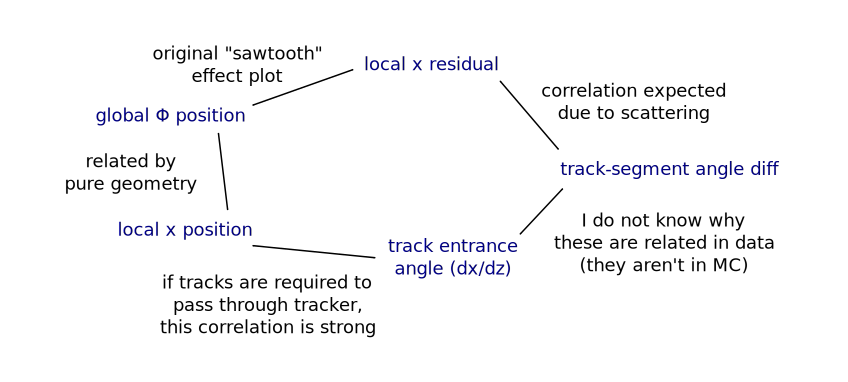
\includegraphics[width=1.2\linewidth]{map_of_correlations.pdf}
\end{frame}

\begin{frame}
\frametitle{1. Recast in local variables}

\includegraphics[width=0.85\linewidth]{map_of_correlations2.pdf}

\vspace{-1 cm}
\begin{columns}
\column{0.55\linewidth}
\begin{itemize}
\item Simple profile plots \\ (each bin is a vertical mean)
\item $p_T > 40$~GeV
\item \textcolor{red}{Red cosmic ray data,} \\ \textcolor{blue}{blue collisions MC} (sorry)
\end{itemize}

\column{0.45\linewidth}
\includegraphics[width=\linewidth]{original_sawtooth.pdf}
\end{columns}
\end{frame}

\begin{frame}
\frametitle{2. Stronger in entrance angle}

\includegraphics[width=0.85\linewidth]{map_of_correlations3.pdf}

\vspace{-1 cm}
\begin{columns}
\column{0.55\linewidth}

\includegraphics[width=0.5\linewidth]{trackangle_correlation.pdf}

\begin{itemize}
\item $x$ and $dx/dz$ are correlated due to globalMuon selection
\begin{itemize}
\item segments may be \mbox{very different\hspace{-1 cm}}
\end{itemize}
\item Residuals trend is twice as strong in $dx/dz$ than in $x$
\end{itemize}

\column{0.45\linewidth}
\includegraphics[width=\linewidth]{vstrackangle_sawtooth.pdf}
\end{columns}
\end{frame}

\begin{frame}
\frametitle{3. Related to known effect?}

\includegraphics[width=0.85\linewidth]{map_of_correlations4.pdf}

\vspace{-1 cm}
\begin{columns}
\column{0.55\linewidth}

\begin{itemize}
\item Same size as correlation between position residual and angle residual
\end{itemize}

\includegraphics[width=\linewidth]{sawtooth_diagram.pdf}

\column{0.45\linewidth}
\includegraphics[width=\linewidth]{understandable_effect.pdf}
\end{columns}
\end{frame}

\begin{frame}
\frametitle{4. Linked through angle error?}

\includegraphics[width=0.85\linewidth]{map_of_correlations5.pdf}

\vspace{-0.75 cm}
\begin{columns}
\column{0.55\linewidth}

\begin{itemize}
\item Roughly the right magnitude to transmit scattering correlation
  to sawtooth
\item Not seen in MC
\item Observed equally in $\pm q$, \\ higher $p_T$ cuts
\item Observable in 2-D distribution
\end{itemize}

\column{0.45\linewidth}
\includegraphics[width=\linewidth]{strange_correlation.pdf}
\end{columns}
\end{frame}

\begin{frame}
\frametitle{5. Seen in new alignment plots}

\begin{columns}
\column{0.4\linewidth}
\begin{itemize}
\item Updated alignment procedure aligns and plots all 6 d.o.f.
\item ``$\phi_y$ residual'' (below) is \mbox{``track-segment angle diff''\hspace{-1 cm}}
\end{itemize}

\column{0.65\linewidth}
\includegraphics[width=\linewidth]{map_of_correlations6.pdf}
\end{columns}

\vfill
\includegraphics[height=\linewidth, angle=90]{possible_acoplanarity.pdf}
\end{frame}

\begin{frame}
\frametitle{Chamber-by-chamber correlation}

\begin{columns}
\column{0.7\linewidth}
\includegraphics[height=\linewidth, angle=90]{possible_acoplanarity.pdf}

\includegraphics[height=\linewidth, angle=90]{DTrphiVsPhi_st1_whC.pdf}

\column{0.4\linewidth}
\begin{itemize}
\item $\phi_y$ effect varies from chamber to chamber, and agrees with original $x$ sawtooth (page~2)
\begin{itemize}
\item last 3 are flatter in both $\phi_y$ residuals and $x$ residuals
\end{itemize}

\item Discontinuities at chamber boundaries indicate a local phenomenon, rather than track source
\begin{itemize}
\item old argument, now applied to $\phi_y$ as well as $x$
\end{itemize}

\end{itemize}
\end{columns}

\end{frame}

\begin{frame}
\frametitle{Sanity checks}

\vspace{0.35 cm}
\begin{tabular}{p{0.5\linewidth} p{0.5\linewidth}}
The $\phi_y$ residual vs.~global $\phi$ plot & Turn off fancy fitting (simple profile)

\vspace{0.05 cm}
{\scriptsize Mean shows the same trends.  Error on mean overestimated due to tails in distribution (that's why we do the fitting).} \\
\vspace{0.01 cm} \includegraphics[height=\linewidth, angle=90]{possible_acoplanarity.pdf} & 
\vspace{0.01 cm} \includegraphics[height=\linewidth, angle=90]{possible_acoplanarity2.pdf} \\

& \\

Antisymmetric ``error tracer''

\vspace{0.05 cm}
{\scriptsize No significant $\vec{B}(\vec{x})$ or $dE/dx$ errors} & Plot in collisions MC, ideal geometry

\vspace{0.05 cm}
{\scriptsize No problems with the technique} \\

\vspace{0.01 cm} \includegraphics[height=\linewidth, angle=90]{possible_acoplanarity3.pdf} & 
\vspace{0.01 cm} \includegraphics[height=\linewidth, angle=90]{possible_acoplanarity_idealmc.pdf} \\
\end{tabular}

\end{frame}

\begin{frame}
\frametitle{New alignment fits}

\begin{itemize}
\item Local $x$, $z$, and $\phi_z$ are aligned in a combined fit (all one fit below)
\item Local $y$ (with redundant $\phi_z$), $\phi_x$, and $\phi_y$ in independent fits
\item Well-understood scattering effect \mbox{controlled as another parameter\hspace{-1 cm}}
\end{itemize}

\includegraphics[width=0.8\linewidth]{example_MBwhCst1sec08.pdf}

\end{frame}

\begin{frame}
\frametitle{Endcap CSC example}

\begin{itemize}
\item Hard to find one with such high statistics
\item Endcaps will be aligned with this tool, using the aligned muon barrel as reference instead of the tracker (reason for the low statistics)
\end{itemize}

\includegraphics[width=0.8\linewidth]{example_MEp22_27.pdf}
\end{frame}

%%%% NO! The plots look like this because you over-wrote the alignment residuals with B-field residuals (which always look good)

%% \begin{frame}
%% \frametitle{Controlling sawtooth}

%% \begin{itemize}
%% \item Fits now contain a term controlling for the scattering effect (correlation between residual position and residual angle), \\ believed to be the cause of the sawtooth effect
%% \item That's why we no longer see the sawtooth shape in alignment plots
%% \item But it's still in track reconstruction, and still not completely understood
%% \end{itemize}

%% \begin{columns}
%% \column{0.6\linewidth}
%% \mbox{ } \hfill Old \hfill \mbox{ }

%% \vspace{0.25 cm}
%% \includegraphics[height=\linewidth, angle=90]{DTrphiVsPhi_st1_whC.pdf}

%% \column{0.6\linewidth}
%% \mbox{ } \hfill New \hfill \mbox{ }

%% \vspace{0.25 cm}
%% \includegraphics[height=\linewidth, angle=90]{example_control_for_sawtooth.pdf}
%% \end{columns}
%% \end{frame}

\begin{frame}
\frametitle{Possible cause of the correlation}

\begin{itemize}
\item The mystery can be restated as: ``why is the error in track entrance
  angle (track-segment angle difference) related to the value of track
  entrance angle?''
\item A guess: could one superlayer be stretched, and not the other? (maybe that has already been ruled out?)

\mbox{ } \hfill \includegraphics[width=0.3\linewidth]{pure_speculation.pdf} \hfill \mbox{ }

\item We now control for the well-understood scattering effect \mbox{in alignment\hspace{-1 cm}}
\begin{itemize}
\item if that's the source of the large residuals, as it seems, then they can no longer affect alignment
\item however, they're still in track-reconstruction
\end{itemize}
\end{itemize}
\end{frame}

\begin{frame}
\frametitle{Alignment schedule}

\begin{itemize}
\item New methods to fit all 6 d.o.f.\ have been implemented (in 3\_1\_X)
\item Studied with high-statistics Monte Carlo (barrel and endcap)
\begin{itemize}
\item may have found a SteppingHelixPropagator bug affecting station~1, wheels~$\pm$2 (highest $\eta$ corner of barrel)
\item need to re-check with 3\_1\_X SteppingHelixPropagator updates
\end{itemize}
\item Re-aligned CRAFT data, looking over results now
\begin{itemize}
\item will probably require small corrections before sign-off
\end{itemize}
\item In $\sim$2 weeks, coordinate with tracker alignment to provide coherent tracker and muon alignments to re-process tracker-pointing skim
\item Use globally-aligned DT chambers as a reference to align as many DTs as possible
\item Use aligned barrel as a reference to align endcap CSCs
\item Re-processing of whole CRAFT dataset would then make sense
\begin{itemize}
\item this end-deadline should be sufficiently before CRAFT-2009
\end{itemize}
\end{itemize}

\end{frame}

%% \begin{frame}
%% \frametitle{Outline}
%% \begin{itemize}\setlength{\itemsep}{0.75 cm}
%% \item 
%% \end{itemize}
%% %% \hspace{-0.83 cm} \textcolor{darkblue}{\Large Outline2}
%% \end{frame}

%% \section*{First section}
%% \begin{frame}
%% \begin{center}
%% \Huge \textcolor{blue}{First section}
%% \end{center}
%% \end{frame}

\begin{frame}
\frametitle{Conclusions}

\begin{itemize}\setlength{\itemsep}{0.25 cm}
\item Some progress in understanding sawtooth effect
\item Not complete (Paolo, Pablo, Ugo, Francesca, Alicia, and Anna are doing a more extensive study)
\item New alignment plots shed some light on the same issues
\end{itemize}

\label{numpages}
\end{frame}

\end{document}
